\documentclass{article}
\usepackage[utf8]{inputenc}
\usepackage{longtable}
\usepackage{authblk}
\usepackage{adjustbox}
\usepackage{natbib}
\usepackage{caption}
\captionsetup[table]{name=Tabla}

\UseRawInputEncoding

\title{Indices de desarrollo humano en Colombia}
% autores
\renewcommand\Authand{, y }
\author[1]{\normalsize David Pulido Suarez}
\author[2]{\normalsize Luis Diaz Bautista}

\affil[1,2]{\small  Facultad de Ingenier\'ia,Universidad de los Andes\\
\texttt{{ds.pulido10,lc.diaz12}@uniandes.edu.col}}
%\affil[1]{\small Instituto de altas investigaciones financieras\\
%Banco del Parque\\
%\texttt{delcurso@bp.com.col}}

\date{29 de Junio de 2018}

%%%%
\usepackage{Sweave}
\begin{document}
\Sconcordance{concordance:ProyectoFinal.tex:ProyectoFinal.Rnw:%
1 26 1 1 0 32 1}


\maketitle


\begin{abstract}
Este es mi primer trabajo en exploraci\'on y modelamiento de indices usando LATEX. Este trabajo lo he hecho bajo la filosof\'ia de trabajo replicable con la integraci\'on de herramientas como python, R, zotero , github y LATEX. 
\end{abstract}

\section*{Introducci\'on}

Aqu\'i les presento mi investigaci\'on sobre diversos indices sociales en Colombia. Los indices los consegu\'i de el curso dictado por \textbf{\cite{magallanes}}, espero que les gusten mucho. Etiam porttitor vel sem dapibus euismod. Sed eu nunc vestibulum, sodales arcu id, lacinia odio. Donec sit amet justo ac lorem condimentum ultricies. Sed nec convallis libero, a porttitor neque. Praesent suscipit consectetur arcu non sollicitudin. Morbi et auctor lorem, id eleifend purus. Nulla nec consectetur sapien, id dictum magna. Duis suscipit urna quis facilisis tincidunt. Duis consectetur ac libero a commodo. Vivamus augue dui, mollis quis dictum sodales, accumsan sed magna. Nunc et odio leo.

Maecenas et nunc eget quam pretium malesuada id at nisi. Praesent facilisis, enim sit amet convallis sodales, tellus arcu molestie odio, eu mattis turpis mi eget sapien. Fusce ut mi velit. Pellentesque habitant morbi tristique senectus et netus et malesuada fames ac turpis egestas. Maecenas consequat, libero non semper lacinia, nunc diam mollis orci, sit amet vehicula elit mi non ex. Nulla blandit, dui quis aliquet maximus, justo felis sollicitudin velit, at condimentum est ipsum efficitur elit. Vestibulum quam elit, aliquam quis laoreet quis, porta vel lorem. Vestibulum sagittis dui libero, venenatis commodo sem porta ut. Suspendisse eget convallis tellus, viverra commodo mi. Maecenas pretium efficitur sodales. Morbi pretium eu erat a imperdiet. Vivamus et vulputate nisi.

Comencemos viendo que hay en la secci\'on \ref{univariada} en la p\'agina \pageref{univariada}.

\clearpage
\section{Exploraci\'on Univariada}\label{univariada}
En esta secci\'on se analiza cada \'indice. Morbi accumsan nec est ut malesuada. Donec metus augue, commodo eget leo et, sodales vulputate libero. Donec eu sollicitudin ligula. Quisque tempor, tellus ultricies vestibulum suscipit, leo dui porta lectus, sed viverra quam est vitae nunc. In vehicula risus ac nibh tempor vehicula. Donec ut finibus nisi, non ullamcorper neque. Vivamus eget viverra metus. Sed hendrerit ipsum porta tellus condimentum facilisis. Nulla eros neque, commodo at tincidunt vitae, fringilla nec nunc. Pellentesque eleifend suscipit ipsum vitae efficitur. Aenean at sem et mi ultrices faucibus en la Tabla \ref{stats}.


% Table created by stargazer v.5.2.2 by Marek Hlavac, Harvard University. E-mail: hlavac at fas.harvard.edu
% Date and time: jue., jul. 05, 2018 - 3:51:19 p.m.
\begin{table}[!htbp] \centering 
  \caption{Medidas estadisticas de los datos} 
  \label{stats} 
\begin{tabular}{@{\extracolsep{5pt}}lccccc} 
\\[-1.8ex]\hline 
\hline \\[-1.8ex] 
Statistic & \multicolumn{1}{c}{N} & \multicolumn{1}{c}{Mean} & \multicolumn{1}{c}{Median} & \multicolumn{1}{c}{Min} & \multicolumn{1}{c}{Max} \\ 
\hline \\[-1.8ex] 
IDH & 32 & 0.802 & 0.804 & 0.691 & 0.879 \\ 
Poblacion.Cabecera & 32 & 1,196,730.000 & 717,197 & 13,090 & 10,070,801 \\ 
Poblacion.Resto & 32 & 360,590.300 & 268,111.5 & 21,926 & 1,428,858 \\ 
Poblacion.Total & 32 & 1,557,320.000 & 1,028,429 & 43,446 & 10,985,285 \\ 
\hline \\[-1.8ex] 
\end{tabular} 
\end{table} A continuaci\'on se muestra el histograma para el \'indice de desarrollo humano en Colombia. (Ver figura \ref{barplot1})
\begin{figure}[h]
\centering
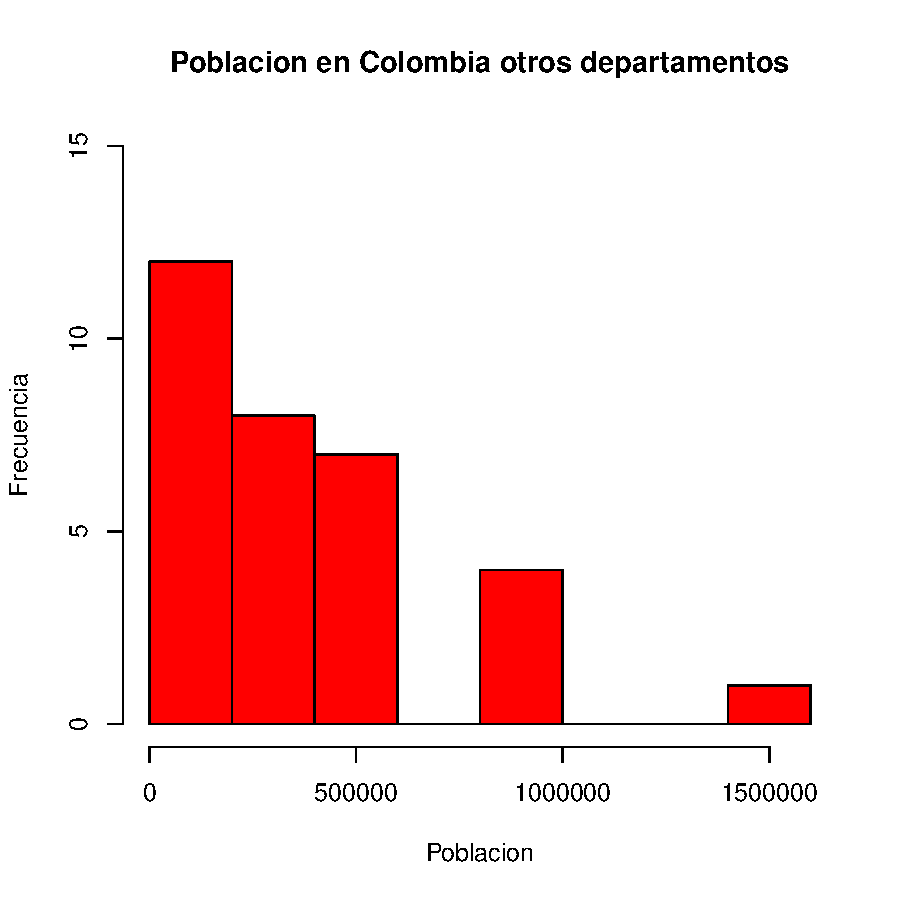
\includegraphics{univariada-summaryDatos}
\caption{Histograma del IDH en Colombia para los 32 departamentos}
\label{barplot1}
\end{figure}

En la figura \ref{barplot2} se muestra el histograma para la cantidad de habitantes en los departamentos de cabecera, mientras que en la figura \ref{barplot3} se muestra la poblaci\'on para el resto de departamentos.
 
\begin{figure}[h]
\centering
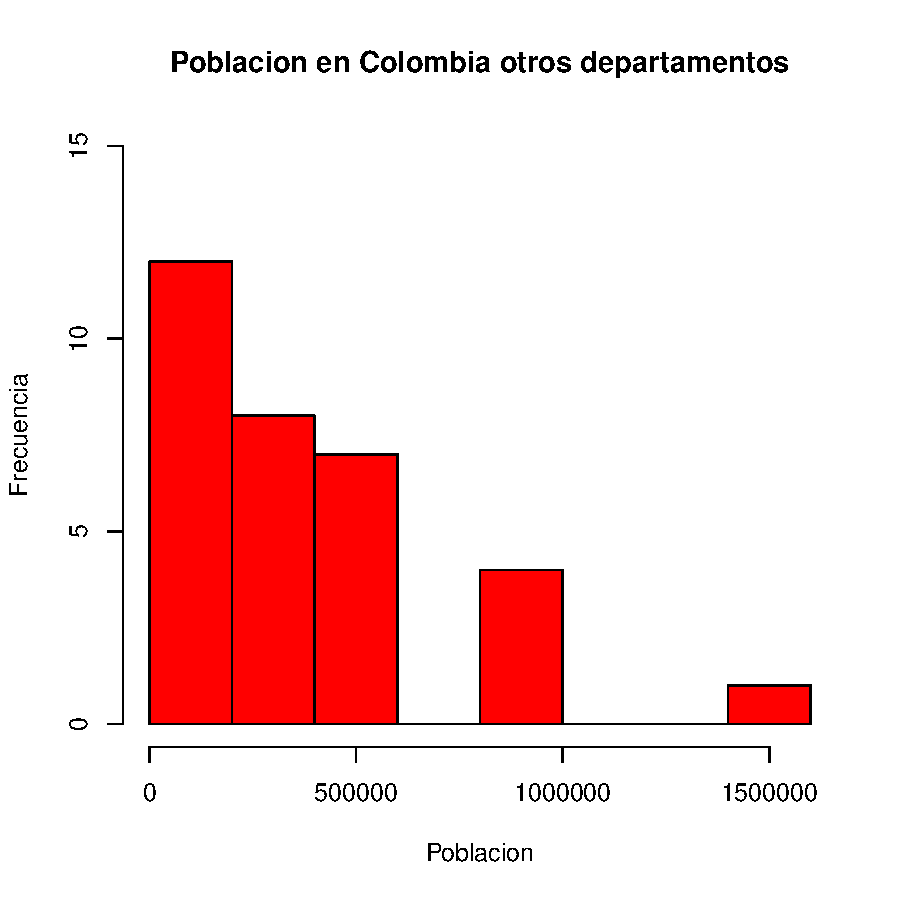
\includegraphics{univariada-summaryDatos}
\caption{Histograma de la poblacion en Colombia para los departamentos de cabecera}
\label{barplot2}
\end{figure}
\begin{figure}[h]
\centering
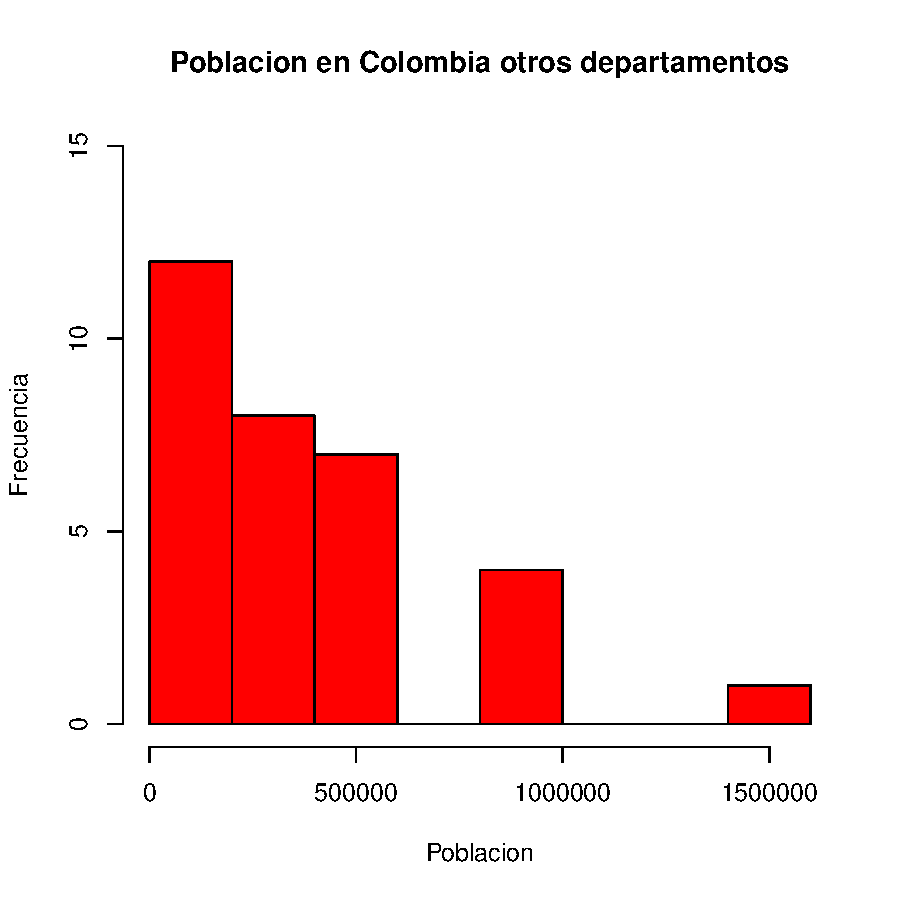
\includegraphics{univariada-summaryDatos}
\caption{Histograma de la poblacion en Colombia para los otros departamentos}
\label{barplot3}
\end{figure}
Los histogramas de los datos del indice se muestran en las figuras 
\begin{figure}[h]
\centering

dado el sesgo de las poblaciones, se realiza una transformaci�n de tal manera que se acerque a la realidad. En la figura \ref{barplot4} se muestra el resultado de esta transformaci\'on.

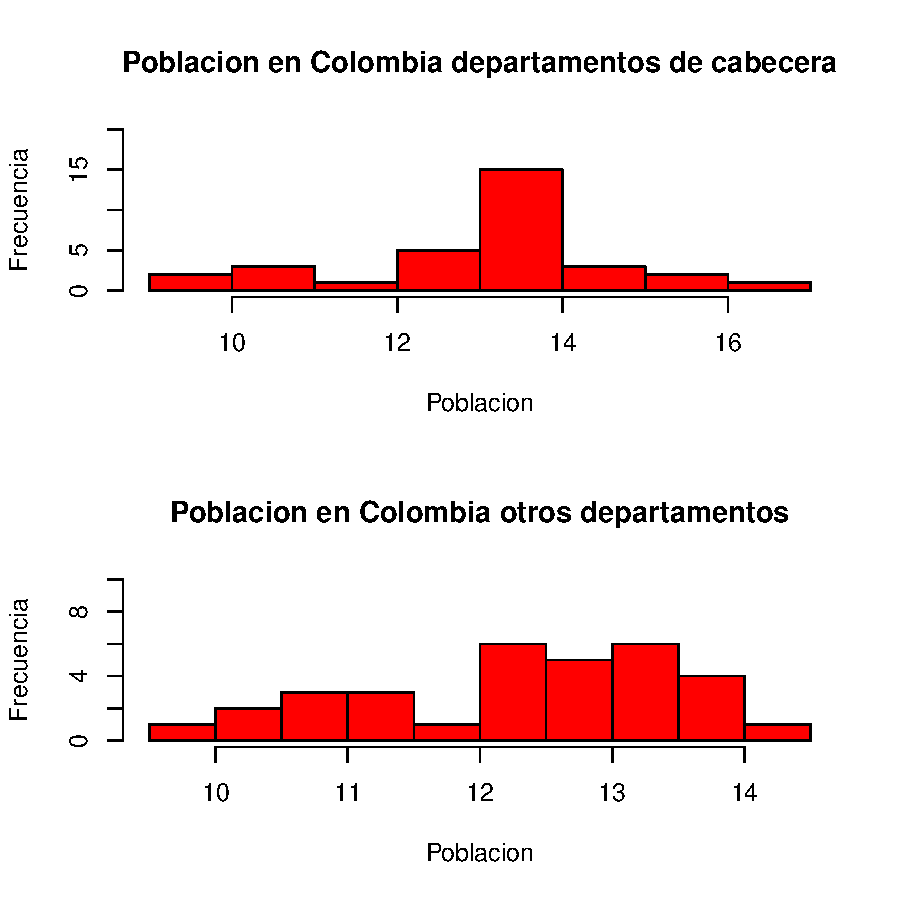
\includegraphics{univariada-rehacerhistogramas}
\caption{Histograma transformado de la poblacion en Colombia para los 32 departamentos}
\label{barplot4}
\end{figure}

\clearpage

\section{Exploraci\'on Bivariada}

En este trabajo estamos interesados en el impacto de la cantidad de habitantes en el \'indice de desarrollo humano. Veamos las relaciones bivariadas que tiene esta variable con todas las dem\'as:


% Table created by stargazer v.5.2.2 by Marek Hlavac, Harvard University. E-mail: hlavac at fas.harvard.edu
% Date and time: jue., jul. 05, 2018 - 6:59:25 p.m.
\begin{table}[!htbp] \centering 
  \caption{Correlacion del IDH con la poblacion} 
  \label{corrDem} 
\begin{tabular}{@{\extracolsep{5pt}} cc} 
\\[-1.8ex]\hline 
\hline \\[-1.8ex] 
cabeLog & restoLog \\ 
\hline \\[-1.8ex] 
$0.487$ & $0.177$ \\ 
\hline \\[-1.8ex] 
\end{tabular} 
\end{table} 
Veamos la correlaci\'on entre las variables independientes:

% Table created by stargazer v.5.2.2 by Marek Hlavac, Harvard University. E-mail: hlavac at fas.harvard.edu
% Date and time: jue., jul. 05, 2018 - 6:59:25 p.m.
\begin{table}[!htbp] \centering 
  \caption{Correlacion entre variables independientes} 
  \label{corrTableX} 
\begin{tabular}{@{\extracolsep{5pt}} ccc} 
\\[-1.8ex]\hline 
\hline \\[-1.8ex] 
 & cabeLog & restoLog \\ 
\hline \\[-1.8ex] 
cabeLog & 1 &  \\ 
restoLog & 0.84 & 1 \\ 
\hline \\[-1.8ex] 
\end{tabular} 
\end{table} 
Lo visto en la Tabla \ref{corrTableX} se refuerza claramente en las figuras \ref{corrPlot} y \ref{corrPlotX}.

\begin{figure}[H]
\centering
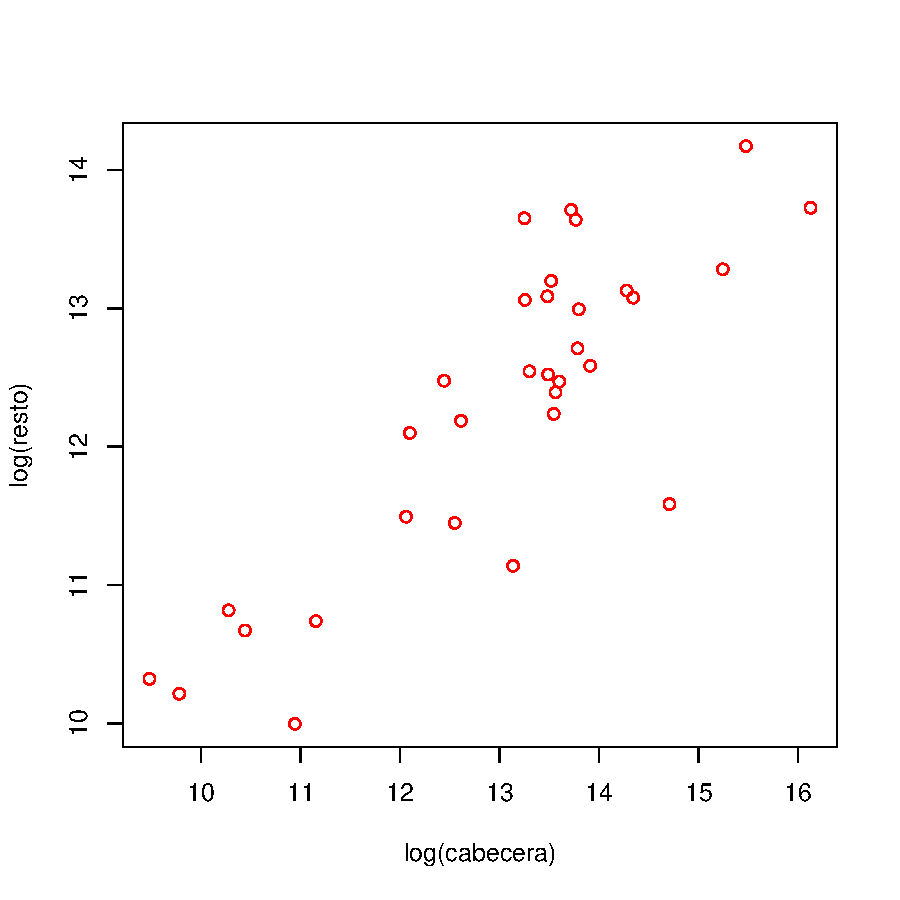
\includegraphics[width=0.7\textwidth]{correlacion-corrPlotX}
\caption{correlacion entre predictores}
\label{corrPlot}
\end{figure}
\endinput
\label{bivariada}



\begin{figure}[h]
\centering
\begin{adjustbox}{width=7cm,height=7cm,clip,trim=1.5cm 0.5cm 0cm 1.5cm}
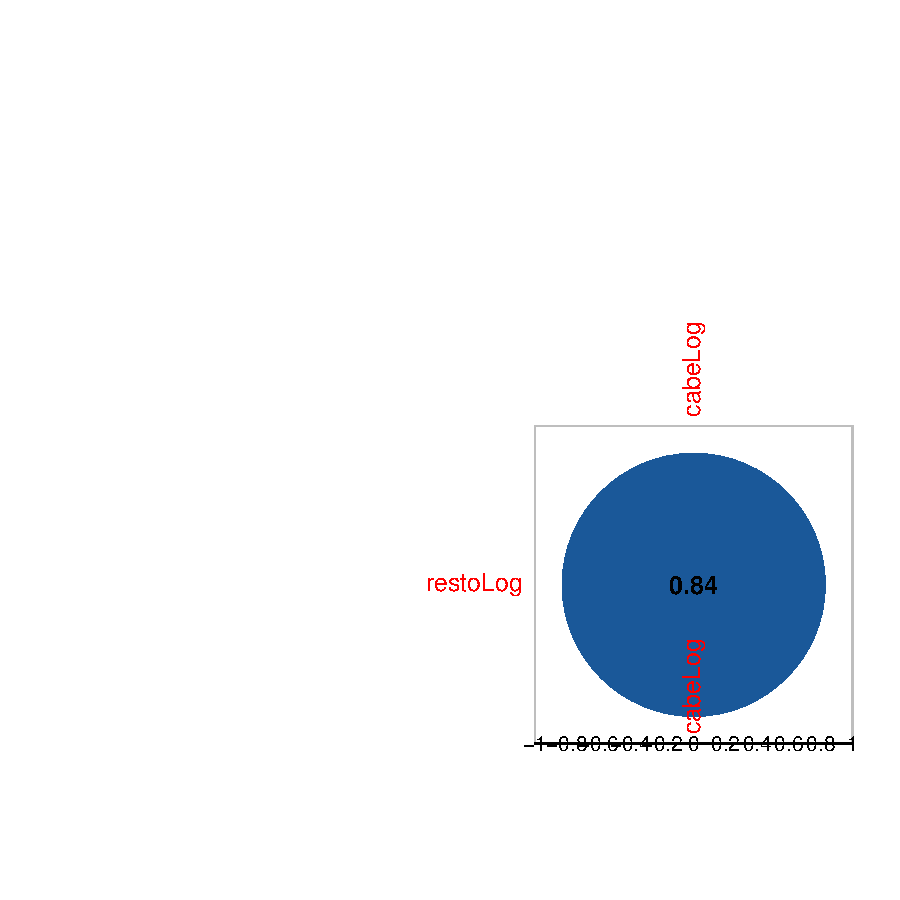
\includegraphics{bivariada-corrPlotX}
\end{adjustbox}
\caption{correlacion entre predictores}
\label{corrPlotX}
\end{figure}


\clearpage


\endinput

\clearpage
\section{Modelos de Regresion}

Finalmente, vemos los modelos propuestos. Primero sin la libertad mundial como independiente, y luego con est\'a. Los resultados se muestran en la tablas \ref{regresiones} y \ref{regresiones1} de la p\'agina \pageref{regresiones} y \pageref{regresiones1}.

\begin{table}[H] \centering 
  \caption{Modelo de regresi\'on propuesto para los datos de departamentos de cabecera} 
  \label{regresiones} 
\begin{tabular}{@{\extracolsep{5pt}}lc} 
\\[-1.8ex]\hline 
\hline \\[-1.8ex] 
 & \multicolumn{1}{c}{\textit{Dependent variable:}} \\ 
\cline{2-2} 
\\[-1.8ex] & IDH \\ 
\hline \\[-1.8ex] 
 cabeLog & 0.013$^{***}$ \\ 
  & (0.004) \\ 
  & \\ 
 Constant & 0.634$^{***}$ \\ 
  & (0.055) \\ 
  & \\ 
\hline \\[-1.8ex] 
Observations & 32 \\ 
R$^{2}$ & 0.238 \\ 
Adjusted R$^{2}$ & 0.212 \\ 
Residual Std. Error & 0.037 (df = 30) \\ 
F Statistic & 9.347$^{***}$ (df = 1; 30) \\ 
\hline 
\hline \\[-1.8ex] 
\textit{Note:}  & \multicolumn{1}{r}{$^{*}$p$<$0.1; $^{**}$p$<$0.05; $^{***}$p$<$0.01} \\ 
\end{tabular} 
\end{table} 

Cras mattis, quam cursus pellentesque efficitur, metus nisi pharetra ipsum, blandit bibendum purus lacus nec enim. Vestibulum leo dui, ultrices et nibh a, accumsan finibus elit. Duis pellentesque ligula a justo volutpat dapibus. Donec in ligula eget ante aliquet convallis. Curabitur placerat nisi at justo euismod elementum. Fusce tristique risus pulvinar turpis interdum ultrices. Vivamus luctus congue dapibus. Nullam et commodo metus. Aenean tincidunt consequat mattis. Nunc ut lectus tempor, pretium nisi quis, pulvinar nisl. Interdum et malesuada fames ac ante ipsum primis in faucibus. Aliquam egestas feugiat turpis congue ullamcorper. Maecenas porta pulvinar erat a aliquet. Mauris scelerisque nibh quis bibendum dictum. Mauris at fringilla leo, vel dapibus ipsum. Pellentesque sit amet ex iaculis elit blandit lobortis.

Interdum et malesuada fames ac ante ipsum primis in faucibus. Proin mauris enim, interdum a tristique in, sagittis nec turpis. Sed in tristique felis, vitae tempus urna. Nulla facilisi. Ut pellentesque libero quis vulputate porta. Cras vitae risus est. In hac habitasse platea dictumst.

\begin{table}[H] \centering 
  \caption{Modelo de regresi\'on propuesto para los datos de todos los departamentos} 
  \label{regresiones1} 
\begin{tabular}{@{\extracolsep{5pt}}lc} 
\\[-1.8ex]\hline 
\hline \\[-1.8ex] 
 & \multicolumn{1}{c}{\textit{Dependent variable:}} \\ 
\cline{2-2} 
\\[-1.8ex] & IDH \\ 
\hline \\[-1.8ex] 
 cabeLog & 0.031$^{***}$ \\ 
  & (0.007) \\ 
  & \\ 
 restoLog & $-$0.030$^{***}$ \\ 
  & (0.010) \\ 
  & \\ 
 Constant & 0.766$^{***}$ \\ 
  & (0.065) \\ 
  & \\ 
\hline \\[-1.8ex] 
Observations & 32 \\ 
R$^{2}$ & 0.425 \\ 
Adjusted R$^{2}$ & 0.385 \\ 
Residual Std. Error & 0.033 (df = 29) \\ 
F Statistic & 10.706$^{***}$ (df = 2; 29) \\ 
\hline 
\hline \\[-1.8ex] 
\textit{Note:}  & \multicolumn{1}{r}{$^{*}$p$<$0.1; $^{**}$p$<$0.05; $^{***}$p$<$0.01} \\ 
\end{tabular} 
\end{table} 

\clearpage
\section{Exploraci\'on espacial}

Como acabamos de ver en la Tabla \ref{regresiones} en la p\'agina \pageref{regresiones}, si quisieras sintetizar la multidimensionalidad de nuestros indicadores, podr\'iamos usar tres de las cuatro variables que tenemos (un par de las originales tiene demasiada correlaci\'on). 

As\'i, propongo que calculemos conglomerados de departamentos usando toda la informaci\'on de tres de los indicadores. Como nuestras variables son ordinales utilizaremos un proceso de conglomeraci\'on usando la tecnica de k-means propuesta por \textbf{\cite{macqueen_methods_1966}}.El resultado de este proceso se muestra en la Figura \ref{mapa}. 

\begin{figure}[H]
\centering
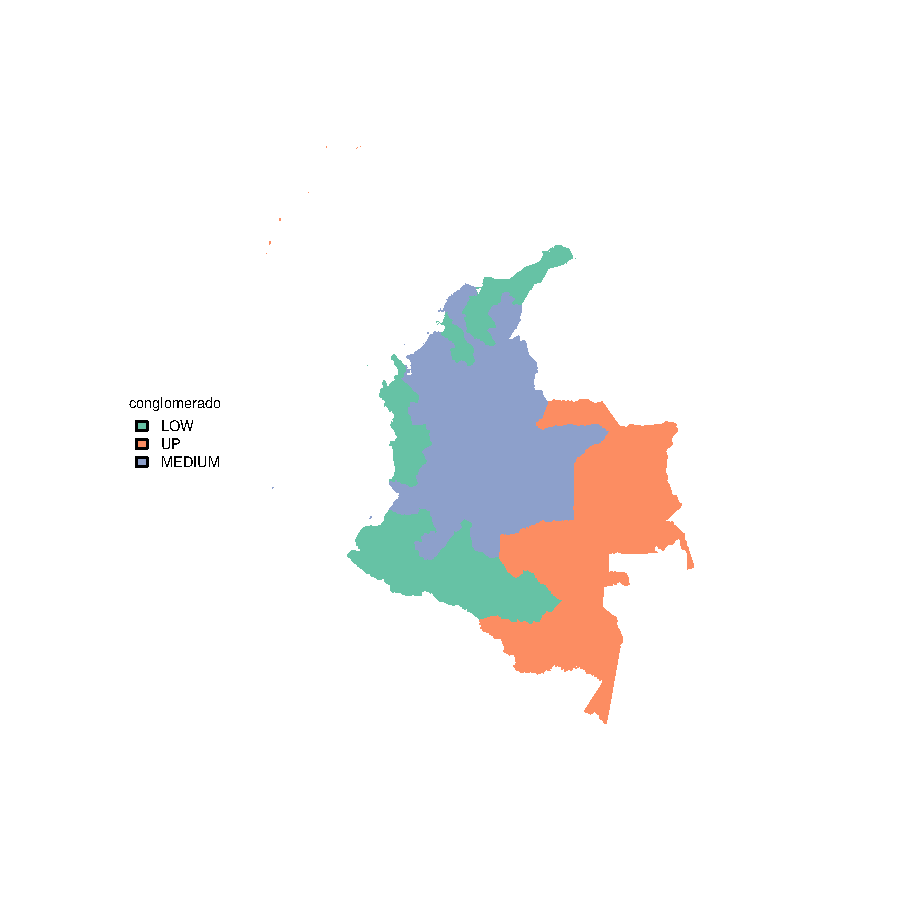
\includegraphics[width=\textwidth,trim={2cm 2cm 3cm 3cm},clip]{Modelos_regresion-plotMap1}
\caption{Histograma del IDH en Colombia para los 32 departamentos}
\label{mapa}
\end{figure}
\endinput

\clearpage
\bibliographystyle{apalike}
\renewcommand{\refname}{Referencias}
\bibliography{colombia}


\end{document}
